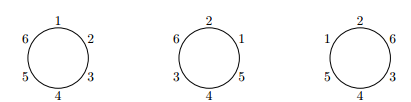
\includegraphics{birthday.png}

The left figure shows the initial arrangement of the children. The middle figure shows the result of the
following reseating: children number 1 and 2 move one place, children number 3 and 5 move two places,
and children number 4 and 6 do not change places. The conditions of arrangement are fulfilled, since 3 sits
between 6 and 4, 4 sits between 3 and 5, 5 sits between 4 and 1, 1 sits between 5 and 2, 2 sits between 1 and
6, and 6 sits between 2 and 3. There exists another possible final arrangement of children, depicted in the
right figure. In both cases no child moves more than two seats.
